\section{TRM minimal: main Nanda-grade result}

TRM minimal is our primary mechanistic target: a recursive variant that can form a Nanda-style sparse Fourier circuit on modular addition.

\paragraph{Multi-seed summary.}
Table~\ref{tab:main_results} reports mean$\pm$std over $\BMINSeeds$ seeds at the analyzed final checkpoint.
Table~\ref{tab:checkpoint_compare} adds grokking- and best-FVE-selected checkpoints from the logged training history.
Final-checkpoint faithful FVE is $\HybridMinimalFVE$; best-FVE across seeds averages $\HybridMinimalFVEBest$ (seed~0 peak: $\HybridMinimalFVESeedZero$).

\paragraph{Progress measures and phases.}
Figure~\ref{fig:phase} shows the Nanda-style phase plot: total squared weight norm, restricted/excluded test CE, embedding Gini, and faithful FVE vs.\ training step.
Restricted trig loss approaches full loss before the test-accuracy jump; excluded loss rises when key Fourier components are removed post-grokking.

\subsection{Mechanistic circuit evidence (TRM minimal)}

Following Section~4 of \citet{nanda2023progress}, we reverse-engineer the grokked minimal TRM using $W_L$ Fourier maps, MLP neuron clustering, and attention routing (Figures~\ref{fig:wl}--\ref{fig:attn}).

At the best-FVE checkpoint (seed~0: step~5000, faithful FVE $\approx 0.96$), five key frequencies dominate excluded-loss sensitivity.
Per-neuron tables (Figure~\ref{fig:neuron_hist}) show concentration of MLP units on $\cos/\sin(\omega_k(a+b))$ features.
The all-frequency ablation grid (Figure~\ref{fig:all_freq}) confirms causal dependence on a sparse frequency subset.

\begin{figure}[h]
  \centering
  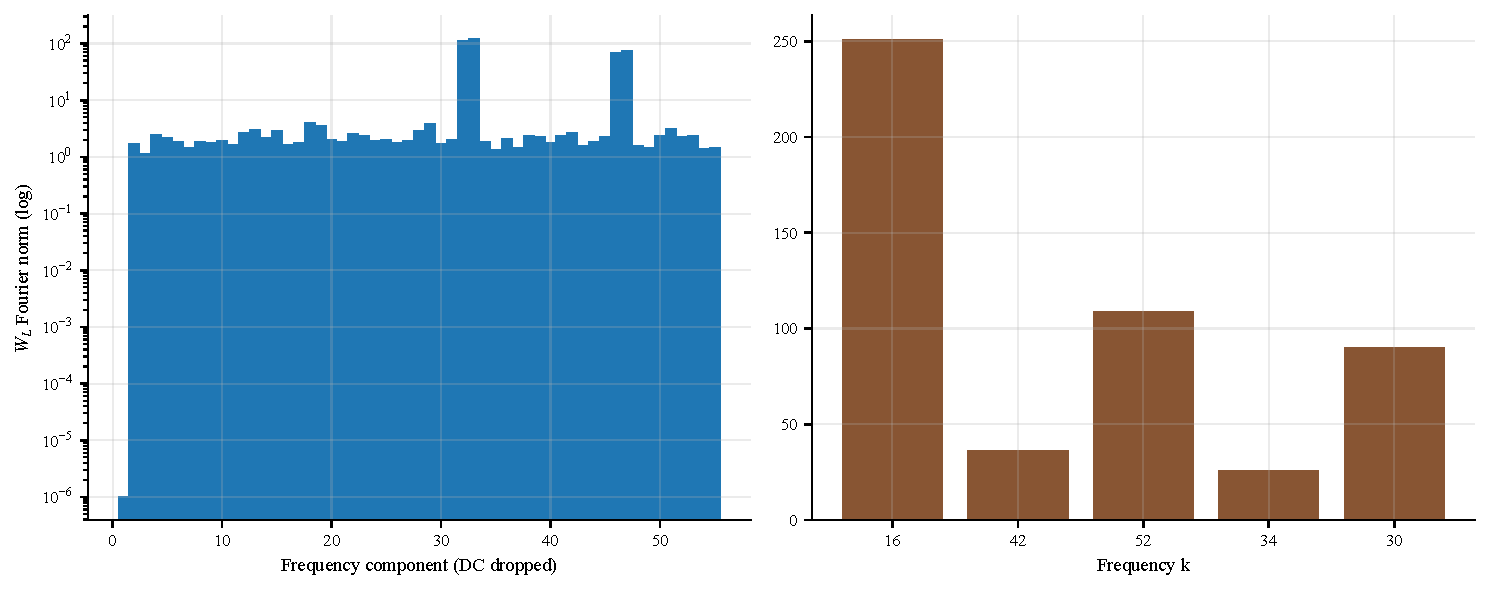
\includegraphics[width=0.95\linewidth]{figures/fig_wl_mlp_reverse_engineering.pdf}
  \caption{$W_L$ Fourier norms and neuron counts per key frequency (TRM minimal seed~0).}
  \label{fig:wl}
\end{figure}

\begin{figure}[h]
  \centering
  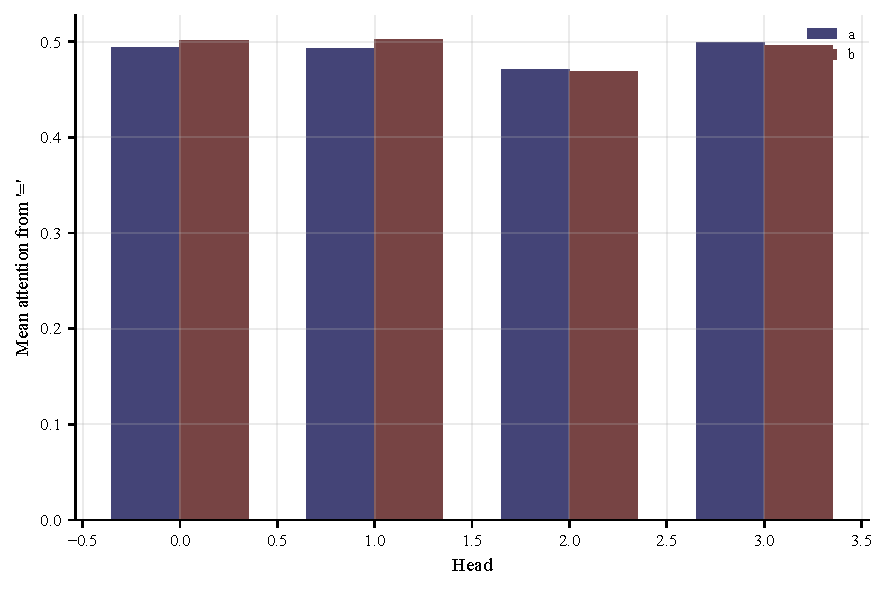
\includegraphics[width=0.7\linewidth]{figures/fig_attention_decomposition.pdf}
  \caption{Attention from ``$=$'' to operand tokens (layer~0).}
  \label{fig:attn}
\end{figure}

\begin{figure}[h]
  \centering
  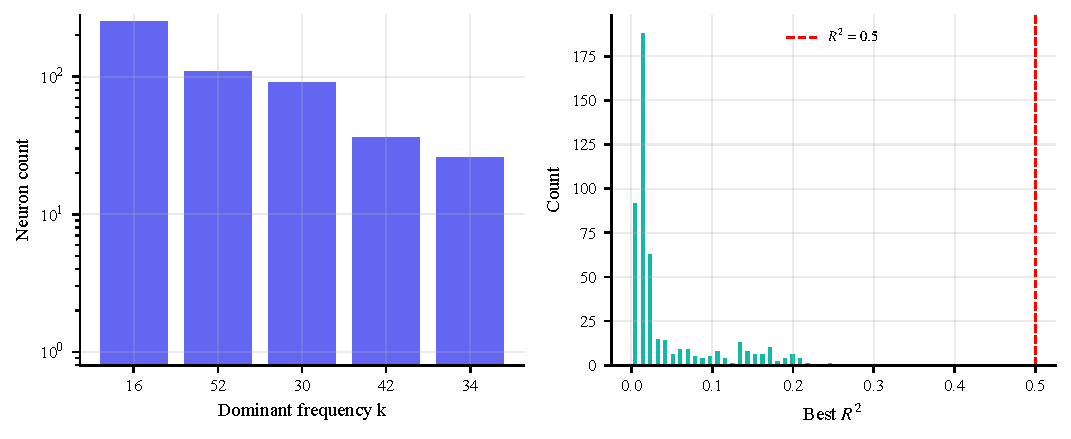
\includegraphics[width=0.95\linewidth]{figures/fig_neuron_frequency_tables.pdf}
  \caption{Per-neuron dominant frequency histogram and $R^2$ distribution.}
  \label{fig:neuron_hist}
\end{figure}

\paragraph{Seed variance diagnosis.}
Multi-seed training reveals that final-checkpoint FVE can collapse during the cleanup phase even when test accuracy remains at 100\% (Table~\ref{tab:seed_variance}, Appendix~\ref{app:seeds}).
We therefore report \textbf{three checkpoint types}: final, first grokking ($\geq 99\%$ acc, low loss), and best faithful FVE among high-accuracy steps (Table~\ref{tab:checkpoint_compare}).
The main Nanda-grade mechanistic claim rests on best-FVE / grokking checkpoints (mean best-FVE FVE $\HybridMinimalFVEBest$), not degraded finals ($\HybridMinimalFVE$).


\begin{figure}[h]
  \centering
  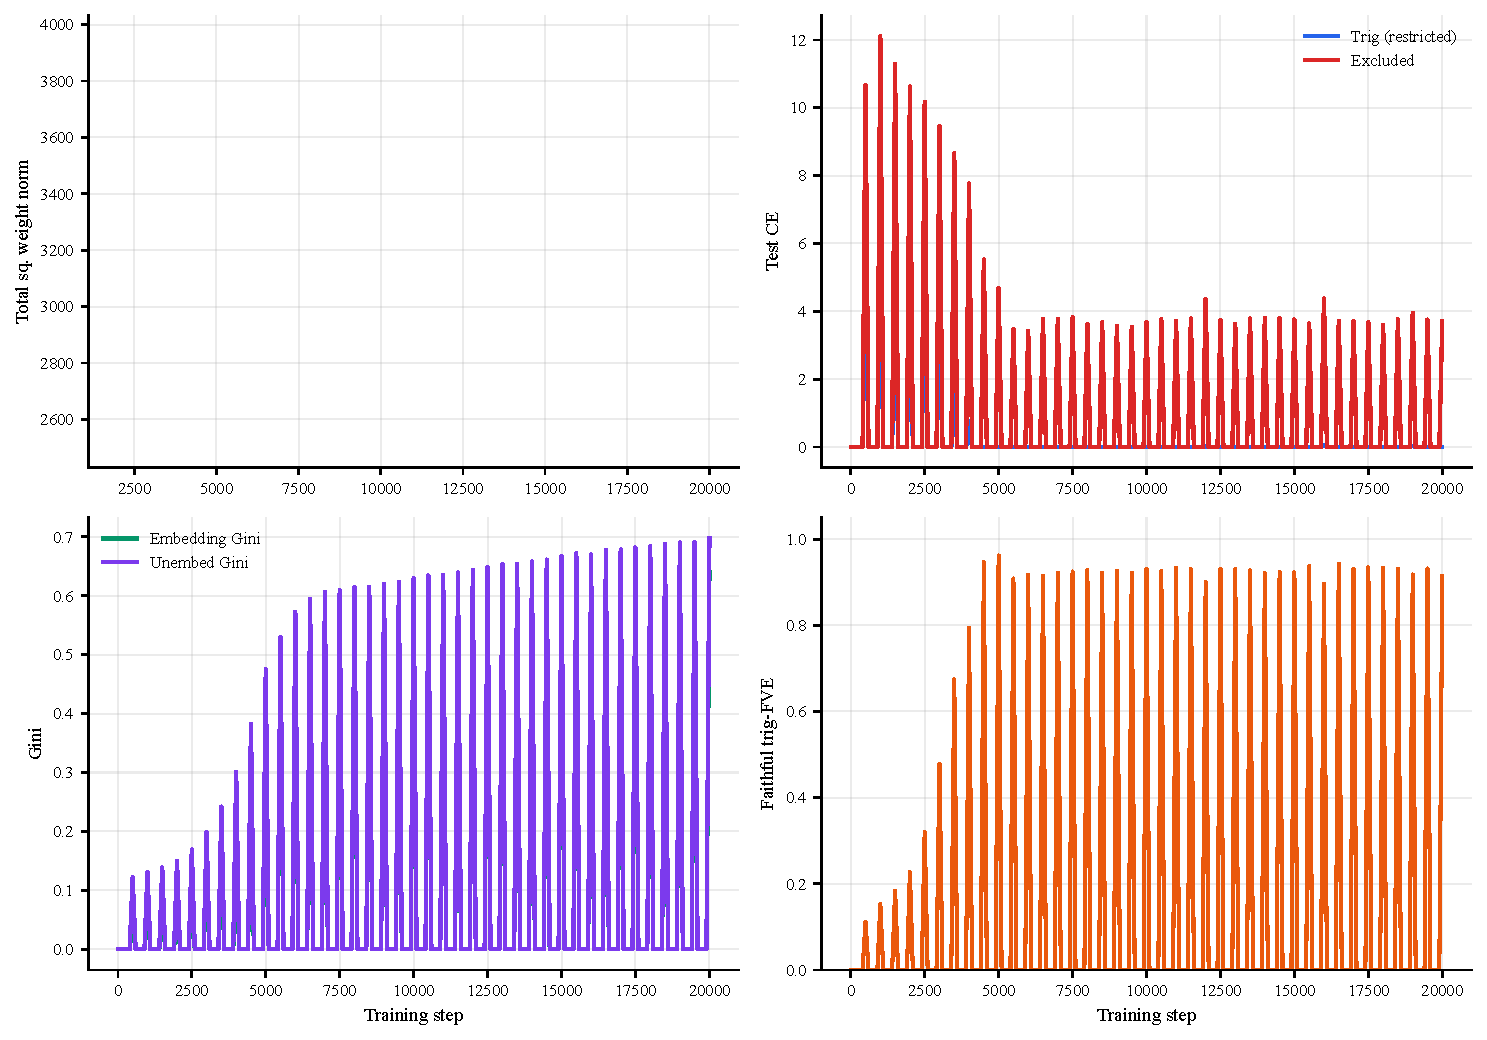
\includegraphics[width=0.95\linewidth]{figures/fig_phase_combined.pdf}
  \caption{Combined grokking phase metrics (TRM minimal seed~0): weight norms, progress measures, Gini, and FVE.}
  \label{fig:phase}
\end{figure}

\begin{figure}[h]
  \centering
  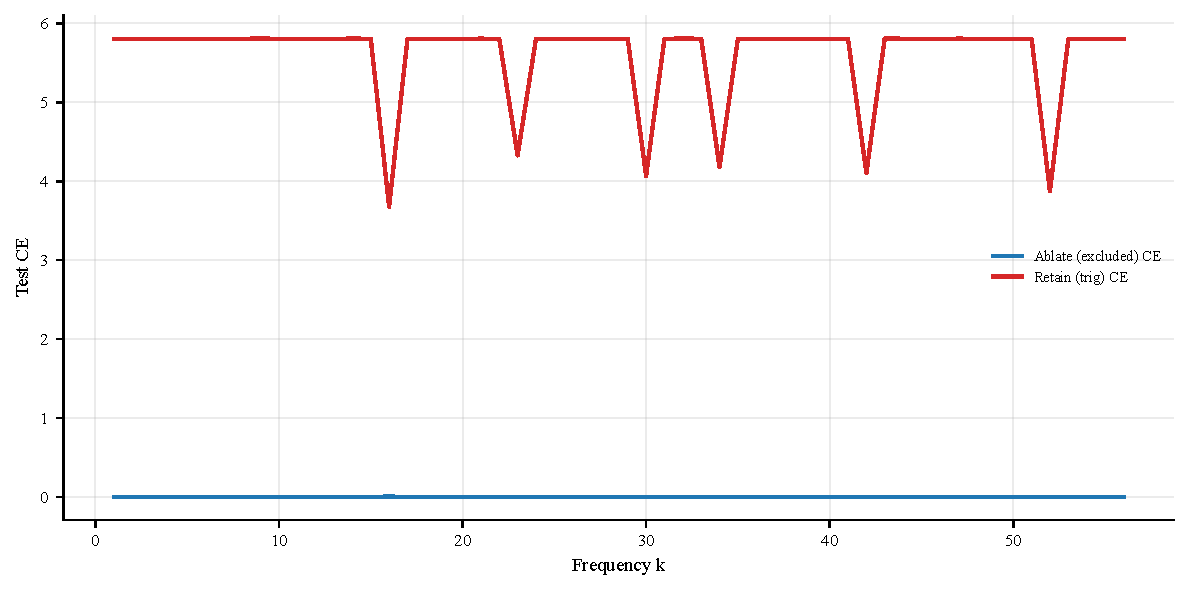
\includegraphics[width=0.95\linewidth]{figures/fig_all_frequency_ablations.pdf}
  \caption{All-frequency retain vs.\ ablate test cross-entropy (TRM minimal seed~0).}
  \label{fig:all_freq}
\end{figure}

\begin{figure}[h]
  \centering
  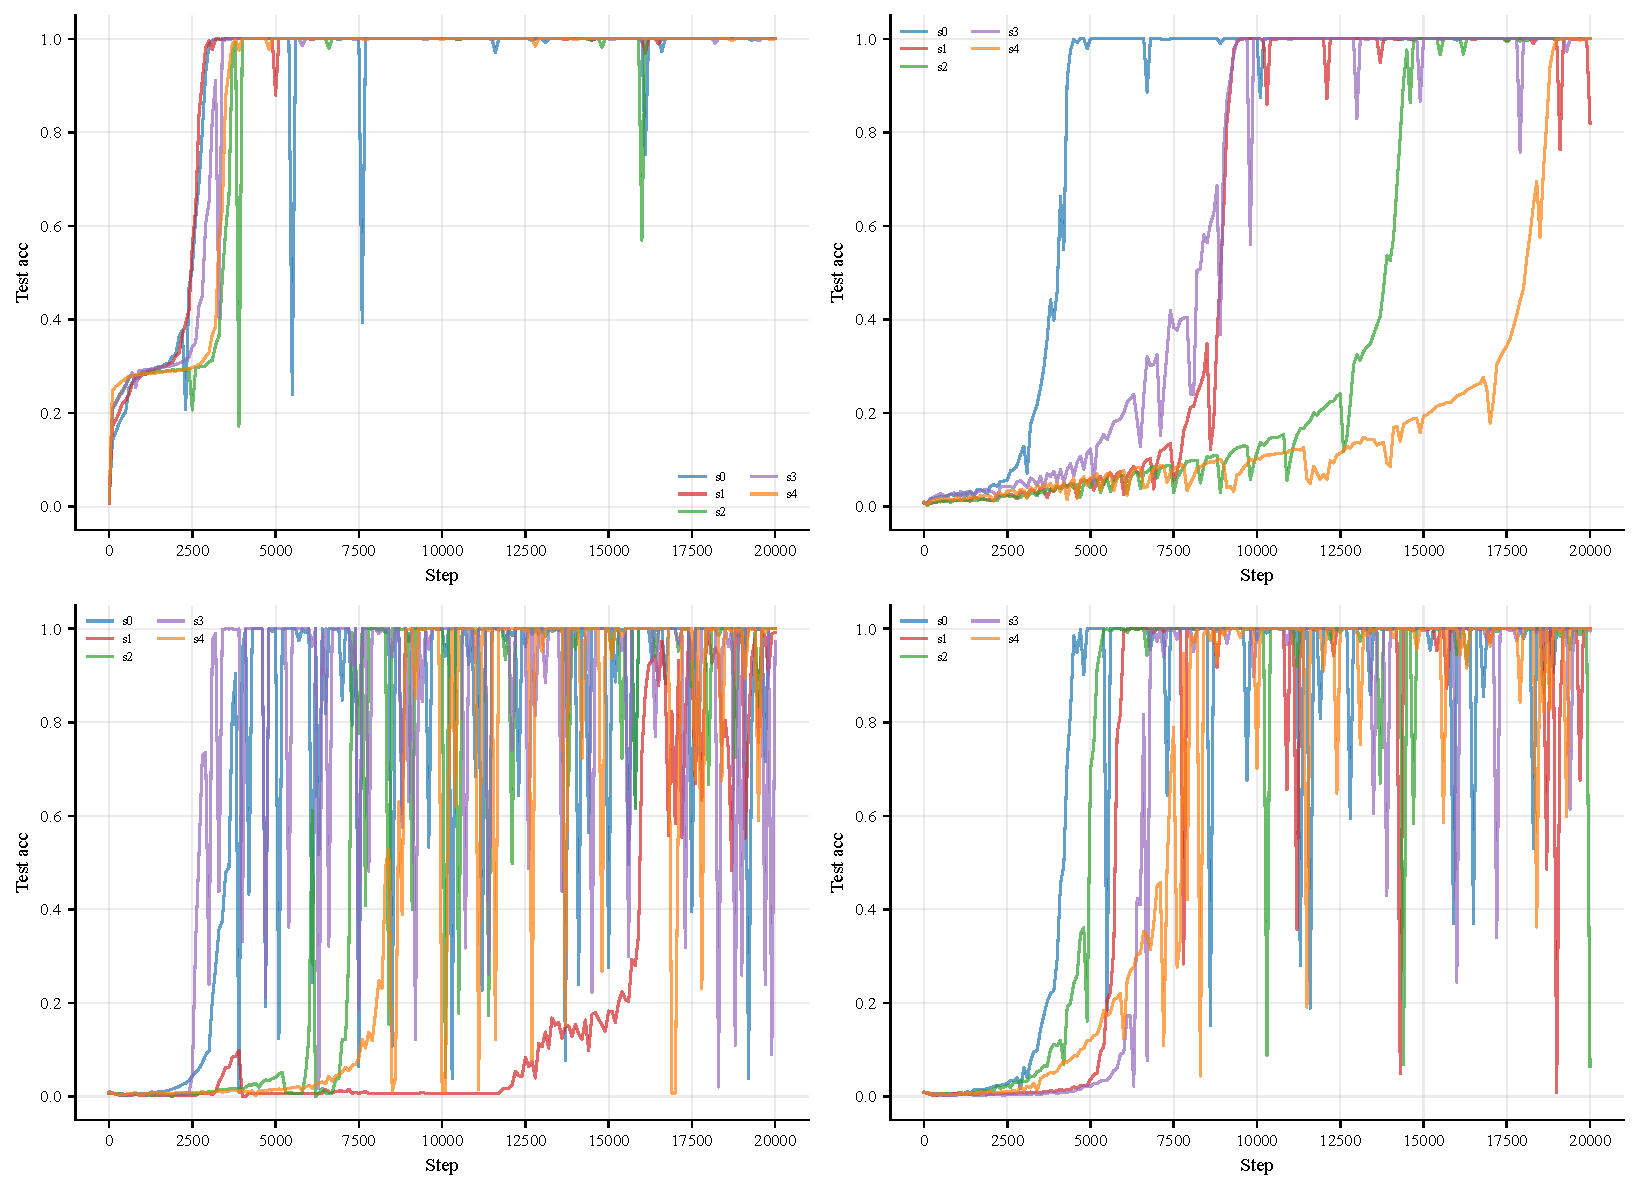
\includegraphics[width=0.95\linewidth]{figures/fig_hybrid_multiseed_grokking.pdf}
  \caption{Per-seed test accuracy trajectories for all four models (50k steps).}
  \label{fig:multiseed_curves}
\end{figure}

\begin{table}[h]
  \centering
  \caption{Checkpoint selection comparison (mean$\pm$std over seeds).}
  \label{tab:checkpoint_compare}
  \begin{tabular}{llrr}
\toprule
Model & Checkpoint & Test Acc. & Faithful FVE \\
\midrule
nanda\_a\_mlp & Final & 1.000 $\pm$ 0.000 & 0.827 $\pm$ 0.045 \\
nanda\_a\_mlp & Grokking & 1.000 $\pm$ 0.001 & 0.349 $\pm$ 0.428 \\
nanda\_a\_mlp & Best FVE & 0.999 $\pm$ 0.001 & 0.888 $\pm$ 0.023 \\
trm\_full\_a & Final & 0.811 $\pm$ 0.374 & 0.393 $\pm$ 0.071 \\
trm\_full\_a & Grokking & 0.998 $\pm$ 0.001 & 0.000 $\pm$ 0.000 \\
trm\_full\_a & Best FVE & 0.999 $\pm$ 0.002 & 0.449 $\pm$ 0.051 \\
trm\_full\_b & Final & 0.953 $\pm$ 0.091 & 0.187 $\pm$ 0.127 \\
trm\_full\_b & Grokking & 0.996 $\pm$ 0.002 & 0.048 $\pm$ 0.095 \\
trm\_full\_b & Best FVE & 0.995 $\pm$ 0.004 & 0.298 $\pm$ 0.117 \\
trm\_minimal & Final & 1.000 $\pm$ 0.000 & 0.509 $\pm$ 0.339 \\
trm\_minimal & Grokking & 0.997 $\pm$ 0.003 & 0.293 $\pm$ 0.384 \\
trm\_minimal & Best FVE & 1.000 $\pm$ 0.000 & 0.786 $\pm$ 0.158 \\
\bottomrule
\end{tabular}

\end{table}

\begin{table}[h]
  \centering
  \caption{TRM minimal seed-variance diagnosis.}
  \label{tab:seed_variance}
  \begin{adjustbox}{max width=\linewidth}
\begin{tabular}{rrrrr p{4cm}}
\toprule
Grok Step & Peak FVE & Peak Step & Final FVE & FVE Drop & Cause \\
\midrule
4500 & 0.962 & 5000 & 0.937 & 0.025 & stable\_\allowbreak circuit \\
9400 & 0.909 & 46500 & 0.907 & 0.002 & stable\_\allowbreak circuit \\
14700 & 0.701 & 14500 & 0.198 & 0.503 & cleanup\_\allowbreak phase\_\allowbreak fve\_\allowbreak collapse \\
9400 & 0.866 & 9000 & 0.272 & 0.594 & cleanup\_\allowbreak phase\_\allowbreak fve\_\allowbreak collapse \\
19000 & 0.558 & 19500 & 0.228 & 0.330 & post\_\allowbreak grokking\_\allowbreak fve\_\allowbreak decay,\allowbreak cleanup\_\allowbreak phase\_\allowbreak fve\_\allowbreak collapse \\
\bottomrule
\end{tabular}
\end{adjustbox}

\end{table}
